\chapter{Taylor series integration} %Last updated 18-05-2016
\label{ch:tsi}

\section{General theory}
\label{sec:genTsiTheory}

\subsection{Workings of \ac{TSI}}
\label{subsec:workTsi}

\subsection{Step-size}
\label{subsec:stepSizeTsi}

\section{Associated equations}
\label{sec:assEq}
In order for \ac{TSI} to be implemented, the state derivatives have to be modelled as a set of continuous functions which are a function of the state only. The state is described in \Cref{eq:state}, where $m_{MAV}$ is the mass of the \ac{MAV} and the subscript $I$ refers to the inertial frame.

\begin{align} \label{eq:state}
\mathbf{r}&=\begin{pmatrix}
x_{I}\\
y_{I}\\
z_{I}\\
\end{pmatrix}
&
\mathbf{V}&=\begin{pmatrix}
V_{x_{I}} \\
V_{y_{I}} \\
V_{z_{I}}\\
\end{pmatrix}
&
m_{MAV}&
\end{align}

The corresponding state derivatives are then described by \Cref{eq:state_derivatives}.

\begin{align} \label{eq:state_derivatives}
\begin{split} 
\dot{x}_{I}&=V_{x_{I}}\\
\dot{y}_{I}&=V_{y_{I}}\\
\dot{z}_{I}&=V_{z_{I}}
\end{split} 
&
\begin{split}
\ddot{x}_{I}&=\dot{V}_{x_{I}}=a_{x_{I}}\\
\ddot{y}_{I}&=\dot{V}_{y_{I}}=a_{y_{I}}\\
\ddot{z}_{I}&=\dot{V}_{z_{I}}=a_{z_{I}}
\end{split}
&
\dot{m}_{MAV}=-\dfrac{T}{g_{0}I_{sp}}
\end{align}

From this point on, the subscript $I$ is omitted, because the state and the state derivatives are always presented in the inertial frame. The accelerations in the x-, y- and z-direction have three contributing components: gravitational acceleration, drag and thrust. The gravitational acceleration can be directly expressed in the inertial frame however, the drag is presented in the body frame and the thrust is expressed in the propulsion frame. Therefore, both the drag and thrust contributions have to be transformed to the inertial frame using transformation matrices. This then results in the expression for the acceleration vector as shown by \Cref{eq:acc}.

\begin{multline} \label{eq:acc}
\begin{pmatrix}
a_{x}\\
a_{y}\\
a_{z}\\
\end{pmatrix}
=
\begin{pmatrix}
-\mu_{M}\dfrac{x}{r^{3}}\\
-\mu_{M}\dfrac{y}{r^{3}}\\
-\mu_{M}\dfrac{z}{r^{3}}\\
\end{pmatrix}+
\Bigg|_{\mathbf{I}}\mathbb{T}_{\mathbf{z}}\left(-\Omega_{M}t_{O}+\omega_{P}\right)\Bigg|_{\mathbf{R}}\mathbb{T}_{\mathbf{z}}\left(-\tau\right)\mathbb{T}_{\mathbf{y}}\left(\dfrac{\pi}{2}+\delta\right)\Bigg|_{\mathbf{V}}\mathbb{T}_{\mathbf{z}}\left(-\chi\right)\mathbb{T}_{\mathbf{y}}\left(-\gamma\right)\Bigg|_{\mathbf{B}}\left[
\begin{pmatrix}
-\dfrac{D}{m_{MAV}}\\
0\\
0\\
\end{pmatrix}
+  \right. \dots \\
\dotsc
 \left.
\Bigg|_{\mathbf{B}}\mathbb{T}_{\mathbf{z}}\left(-\psi_{T}\right)\mathbb{T}_{\mathbf{y}}\left(-\epsilon_{T}\right)\Bigg|_{\mathbf{P}}
\begin{pmatrix}
\dfrac{T}{m_{MAV}}\\
0\\
0\\
\end{pmatrix}
\right]
\end{multline}

It can be seen that this set of equations is a function of the current position and many other parameters. These parameters will all have to be written as a function of the current state. This is done in \Cref{subsec:auxEq} forming auxiliary equations that need to be solved. Then the recurrence relations can be written for the state derivatives and the corresponding auxiliary equations. To avoid lengthy expressions, the set of equations presented in \Cref{eq:acc} and the auxiliary equations are represented using auxiliary functions. Each of the auxiliary functions performs one simple algebraic operation and the collection of these auxiliary functions then form the complete set of recurrence relations using the recurrence relations for the simple algebraic operations. This is all described in \Cref{subsec:recRelAuxFunc}. 


\subsection{Auxiliary equations}
\label{subsec:auxEq}
For the auxiliary equations, a similar notation will be used as shown by \cite{scott2008high}. Here the equations are denoted by $x_{number}$ and the corresponding derivatives $x'_{number}$. This notation will also be used for the current state and the corresponding state derivatives. This way, \Cref{eq:state} can be written as \Cref{eq:stateX} and the corresponding derivatives can be written as presented by \Cref{eq:state_derivativesX}.

\begin{align} \label{eq:stateX}
\begin{split} 
x_{1}&=x\\
x_{2}&=y\\
x_{3}&=z
\end{split} 
&
\begin{split}
x_{4}&=\dot{x}=V_{x}\\
x_{5}&=\dot{y}=V_{y}\\
x_{6}&=\dot{z}=V_{z}
\end{split}
&
x_{7}=m_{MAV}
\end{align}


\begin{align} \label{eq:state_derivativesX}
\begin{split} 
x'_{1}&=x_{4}\\
x'_{2}&=x_{5}\\
x'_{3}&=x_{6}
\end{split} 
&
\begin{split}
x'_{4}&=\dot{V}_{x}=a_{x}=a_{g,x}+a_{D,x}+a_{T,x}\\
x'_{5}&=\dot{V}_{y}=a_{y}=a_{g,y}+a_{D,y}+a_{T,y}\\
x'_{6}&=\dot{V}_{z}=a_{z}=a_{g,z}+a_{D,z}+a_{T,z}
\end{split}
&
x'_{7}=\dot{m}_{MAV}=-\dfrac{T}{g_{0}I_{sp}}
\end{align}

In this case the thrust and specific impulse are constant, which means that $x'_{7}$ is constant and any additional derivative will be zero. Also, neither one of the thrust angles is a function of the state, which means that $a_{T}$, in the body frame, is only a function of $x_{7}$ (also see \Cref{eq:acc}). However, both $a_{g}$ and $a_{D}$ are a function of the position and velocity, where $a_{D}$ is also a function of the \ac{MAV} mass. Furthermore, both the drag and thrust accelerations have to be translated to the inertial frame using five different angles. The transformation from the rotating to the inertial frame is performed using an angle that is a function of time where $t_{O}=t_{0}+t_{current}$ as shown by \Cref{eq:acc}. This leaves 4 angles that are a function of the state. $a_{g}$ will be discussed first, followed by the transformation angles and $a_{D}$ respectively. For the numbering of all the auxiliary equations goes that the order comes from the manner in which they were all written out on paper. This means that sometimes lower number parameters could contain much higher number parameters without the intermediate parameters defined yet. However, these will all be defined eventually.


\subsubsection{Gravitational acceleration}
 \label{subsubsec:tsiGravity} 
 For the gravitational acceleration two auxiliary equations were required since $r=\sqrt{x^{2}+y^{2}+z^{2}}$. The resulting expressions for the gravitational acceleration are shown in \Cref{eq:gravAcc} with the corresponding auxiliary equations and the derivatives defined in \Cref{eq:gravAux}.
 
 \begin{equation} \label{eq:gravAcc}
\begin{split}
a_{g,x} &= -\mu_{M}\dfrac{x_{1}}{r^{3}} = \dfrac{x_{1}}{\left(x_{1}^{2}+x_{2}^{2}+x_{3}^{2} \right)^{3/2}}=-\mu_{M}\dfrac{x_{1}}{x_{9}}\\
a_{g,y} &= -\mu_{M}\dfrac{x_{2}}{r^{3}} = \dfrac{x_{2}}{\left(x_{1}^{2}+x_{2}^{2}+x_{3}^{2} \right)^{3/2}}=-\mu_{M}\dfrac{x_{2}}{x_{9}}\\
a_{g,z} &= -\mu_{M}\dfrac{x_{3}}{r^{3}} = \dfrac{x_{3}}{\left(x_{1}^{2}+x_{2}^{2}+x_{3}^{2} \right)^{3/2}}=-\mu_{M}\dfrac{x_{3}}{x_{9}}
\end{split}
\end{equation}

\begin{align} \label{eq:gravAux}
\begin{split} 
x_{8}&=x_{1}^{2}+x_{2}^{2}+x_{3}^{2}\\
x_{9}&=x_{8}^{3/2}
\end{split} 
&
\begin{split}
x'_{8}&=2x_{1}x_{4}+2x_{2}x_{5}+2x_{3}x_{6}\\
x'_{9}&=\dfrac{3}{2}\dfrac{x_{9}x_{8}'}{x_{8}}
\end{split}
\end{align}
 
 
 \subsubsection{Transformation angles}
 \label{subsubsec:tsiTransAngl}
 The angles required for the transformation to go from the body frame to the reference frame are all written as auxiliary functions. The latitude and longitude can be described using the position vector in the inertial frame, however the transformation from the body frame to the vertical frame is a function of the velocity in the rotational frame. Since the position and velocity in the inertial frame are known (current state) the rotational velocity ($V_{R}$) has to be written as a function of the inertial velocity ($V_{I}$) as visualised by \Cref{fig:rotational_inertial_martian_velocity} and described in \Cref{eq:inVelToRotVel}. This operation is a simple vector operation where $V_{M}$ is the local rotational velocity of Mars.
 
 \begin{figure}[!ht]
\centering
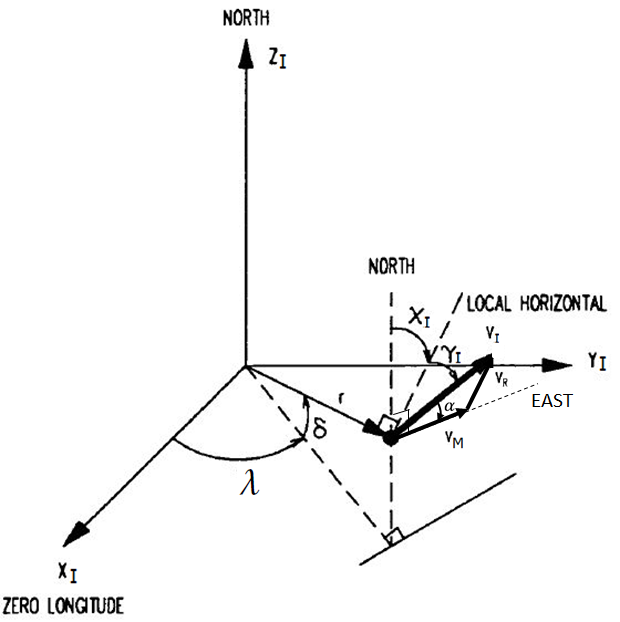
\includegraphics[width=0.7\textwidth]{figures/tsi/rotational_inertial_martian_velocity.png}
\caption{Vector addition of rotational and Martian velocity to form the inertial velocity.}
\label{fig:rotational_inertial_martian_velocity}
\end{figure}
 
\begin{equation} \label{eq:inVelToRotVel}
V_{R} = \sqrt{V_{M}^{2}+V_{I}^{2}-2V_{M}V_{I} \cos\gamma_{I} \sin\chi_{I}}
\end{equation} 
 
The corresponding angles are described using auxiliary equations as defined in \Cref{eq:transAnglAux} resulting from both \Cref{fig:rotational_inertial_martian_velocity,fig:flight_path_and_azimuth_angle}. As was mentioned before, the angle represented by $x_{10}$ is not a function of the state and can therefore be treated as a constant within the current integration step. Also, $t_{0}$ is the time from the moment the inertial frame was set to the start time of the simulation and $t$ is the time from the start of the simulation till the current step, also known as current time. The numbering of the auxiliary equations results from the order in which they were derived.

 \begin{figure}[!ht]
\centering
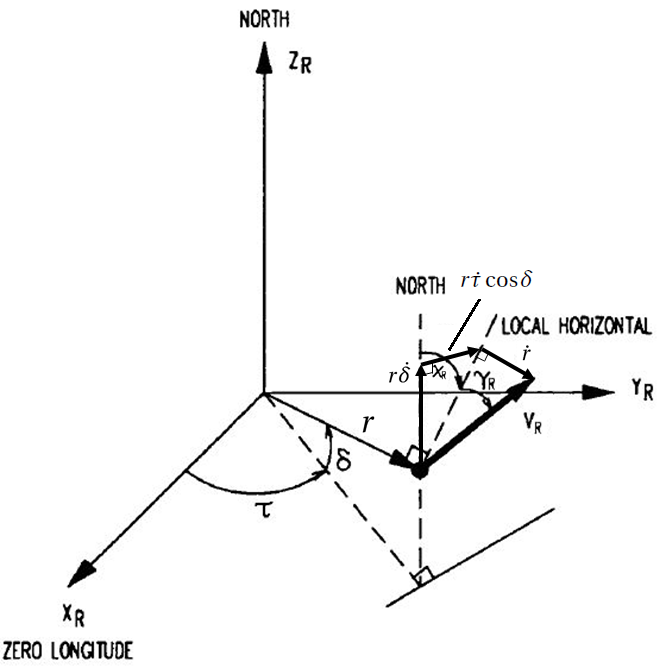
\includegraphics[width=0.7\textwidth]{figures/tsi/flight_path_and_azimuth_angle.png}
\caption{Flight-path and azimuth angle definition in the rotating frame.}
\label{fig:flight_path_and_azimuth_angle}
\end{figure}
 
 \begin{equation} \label{eq:transAnglAux}
\begin{split}
x_{10} &= \Omega_{M}t_{O}-\omega_{P} \quad \text{where} \quad t_{O}=t_{0}+t \\
x_{11} &= \tau = \lambda - x_{10} = \arctan\left(\dfrac{x_{2}}{x_{1}}\right)-x_{10} = \text{atan2}\left(x_{2},x_{1}\right)-x_{10}\\
x_{12} &= \delta = \arcsin\left(\dfrac{x_{3}}{r}\right) = \arcsin\left(\dfrac{x_{3}}{x_{20}}\right)\\
x_{38} &= \gamma_{I} = \arcsin\left(\dfrac{\dot{r}}{V_{I}}\right) = \arcsin\left(x_{37}\right)\\
x_{40} &= \chi_{I} = \arctan\left(\dfrac{\dot{\lambda }\cos\delta}{\dot{\delta}}\right)=\arctan\left(\dfrac{x_{47}}{x_{24}}\right)=\text{atan2}\left(x_{47},x_{24}\right) \\
\end{split}
\end{equation} 

Here the atan2 function is described by the general equations shown in \Cref{fig:atan2_guilhaire2013}.

\begin{figure}[!ht]
\centering
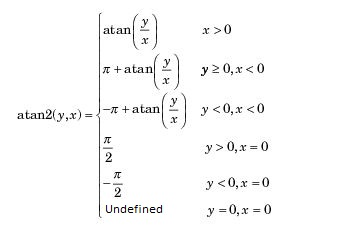
\includegraphics[width=0.5\textwidth]{figures/reference_frames/atan2_guilhaire2013.jpg}
\caption{atan2 function evaluation conditions.}
\label{fig:atan2_guilhaire2013}
\end{figure}

The equations presented in \Cref{eq:transAnglAux} require extra auxiliary equations which are all presented in \Cref{eq:extraTransAnglAux}.
 
 \begin{align} \label{eq:extraTransAnglAux}
\begin{split}
x_{19} &= x_{1}^{2}+x_{2}^{2}\\
x_{20} &= r = \sqrt{x_{8}} \\
x_{21} &= x_{4}^{2}+x_{5}^{2}+x_{6}^{2}\\
x_{24} &= x'_{12} = \dot{\delta} = \dfrac{x_{20}x_{6}-x_{3}x_{25}}{x_{8} \sqrt{1-\left(\dfrac{x_{3}}{x_{20}}\right)^{2}}}\\
x_{25} &= x'_{20}=\dot{r}=\dfrac{x_{26}}{2x_{20}}\\
x_{26} &= x'_{8}=2x_{1}x_{4}+2x_{2}x_{5}+2x_{3}x_{6}\\
\end{split}
&
\begin{split}
x_{35} &= V_{M} = \Omega_{M} x_{20}\cos x_{12}\\
x_{36} &= V_{I} = \sqrt{x_{21}}\\
x_{37} &= \dfrac{x_{25}}{x_{36}}\\
x_{41} &= x_{35}x_{36}\\
x_{42} &= \cos x_{38} \sin x_{40}\\
x_{43} &= x_{41}x_{42}\\
x_{45} &= \dot{\lambda} = \dfrac{x_{1}x_{5}-x_{2}x_{4}}{x_{19}}\\
x_{47} &= x_{45} \cos x_{12} \\
\end{split}
\end{align}  

With the required angles known, \Cref{eq:inVelToRotVel} can be written as an auxiliary function as well including the required transformation angles. These expressions are provided in \Cref{eq:rotTransAnglAux} with the extra auxiliary equations represented by \Cref{eq:rotExtraTransAnglAux}. Here $\dot{\tau}$ was found by noticing that $r\dot{\tau}\cos \delta=r\dot{\lambda}\cos \delta-\Omega_{M}r\cos \delta$, also see \Cref{fig:rotational_inertial_martian_velocity,fig:flight_path_and_azimuth_angle}.

 \begin{equation} \label{eq:rotTransAnglAux}
\begin{split}
x_{15} &= V_{R} = \sqrt{x_{35}^{2}+x_{21}-2x_{43}}\\
x_{14} &= \gamma_{R} = \arcsin\left(\dfrac{\dot{r}}{V_{R}}\right) = \arcsin\left(x_{23}\right)\\
x_{13} &= \chi_{R} = \arctan\left(\dfrac{\dot{\tau}\cos \delta}{\dot{\delta}}\right)=\arctan\left(\dfrac{x_{48}}{x_{24}}\right)=\text{atan2}\left(x_{46},x_{24}\right)\\
\end{split}
\end{equation} 

 
 \begin{align} \label{eq:rotExtraTransAnglAux}
x_{16} &= \cos x_{14}
&
x_{23} &= \dfrac{x_{25}}{x_{15}}
&
x_{46} &= x'_{11} = \dot{\tau} = x_{45}-\Omega_{M}
&
x_{48} &= x_{46}\cos \delta
\end{align}  

The derivatives of all these auxiliary equations are shown in \Cref{eq:derTransAnglAux}.

 \begin{align} \label{eq:derTransAnglAux}
\begin{split}
x'_{10} &= 0 \\
x'_{11} &=  \dot{\tau} = x_{45}-\Omega_{M}\\
x'_{12} &= \dot{\delta} = \dfrac{x_{20}x_{6}-x_{3}x_{25}}{x_{8} \sqrt{1-\left(\dfrac{x_{3}}{x_{20}}\right)^{2}}}\\
x'_{13} &= \dfrac{x_{24}x'_{48}-x_{48}x'_{24}}{x_{48}^{2}+x_{24}^{2}}\\
x'_{14} &= \dfrac{x'_{23}}{\sqrt{1-x_{23}^{2}}}\\
x'_{15} &= \dfrac{2x_{35}x'_{35}+x'_{21}-2x'_{43}}{2x_{15}} \\
x'_{16} &= -\sin x_{14}x'_{14}\\
x'_{19} &= 2x_{1}x_{4}+2x_{2}x_{5}\\
x'_{20} &= \dot{r} = \dfrac{x_{26}}{2 x_{20}}\\
x'_{21} &= 2x_{4}x'_{4}+2x_{5}x'_{5}+2x_{6}x'_{6}\\
x'_{23} &= \dfrac{x_{15}x'_{25}-x_{25}x'_{15}}{x_{15}^{2}}\\
x'_{24} &= x''_{12} = \dfrac{x_{6}x'_{20}+x_{20}x'_{6}-x_{6}x_{25}-x_{3}
x'_{25}}{x_{8}\sqrt{1-\left(\dfrac{x_{3}}{x_{20}}\right)^{2}}}-\\
&\dfrac{\left(\dfrac{2x_{3}^{2}x'_{25}}{x_{20}^{3}}-\dfrac{2x_{3}x_{6}}{x_{8}}\right)\left(x_{20}x_{6}-x_{3}x_{25}\right)}{2x_{8}\left(1-\left(\dfrac{x_{3}}{x_{20}}\right)^{2}\right)^{3/2}}-\dfrac{x'_{8}\left(x_{20}x_{6}-x_{3}x_{25}\right)}{x_{8}^{2}\sqrt{1-\left(\dfrac{x_{3}}{x_{20}}\right)^{2}}}\\
\end{split}
&
\begin{split}
x'_{25} &= x''_{20} = \dfrac{2x_{8}x'_{26}-x_{26}^{2}}{4x_{9}}\\
x'_{26} &= x''_{8} = 2x_{21}+2\left(x_{1}x'_{4}+x_{2}x'_{5}+x_{3}x'_{6}\right)\\
x'_{35} &=  \Omega_{M}\left(\cos x_{12}x_{25}-x_{20}x_{24}\sin x_{12}\right) \\
x'_{36} &=  \dfrac{x'_{21}}{2x_{36}} \\
x'_{37} &= \dfrac{x_{36}x'_{25}-x_{25}x'_{36}}{x_{36}^{2}} \\
x'_{38} &= \dfrac{x'_{37}}{\sqrt{1-x_{37}^{2}}} \\ 
x'_{40} &=  \dfrac{x_{24}x'_{47}-x_{47}x'_{24}}{x_{47}^{2}+x_{24}^{2}}\\
x'_{41} &= x_{36}x'_{35}+x_{35}x'_{36}\\ 
x'_{42} &= \cos x_{38} \cos x_{40} x'_{40}-x'_{38} \sin x_{38} \sin x_{40}\\
x'_{43} &= x_{41}x'_{42}+x_{42}x'_{41} \\ 
x'_{45} &= \dfrac{x_{19}\left(x_{1}x'_{5}-x_{2}x'_{4}\right)-x'_{19}\left(x_{1}x_{5}-x_{2}x_{4}\right)}{x_{19}^{2}}\\
x'_{46} &= x''_{11} = x'_{45} \\
x'_{47} &= x'_{45}\cos x_{12} - x_{45}x'_{12}\sin x_{12} \\
x'_{48} &= x'_{46}\cos x_{12} - x_{46}x'_{12}\sin x_{12} \\
\end{split}
\end{align}

 \subsubsection{Drag acceleration}
 \label{subsubsec:tsiDrag}
The drag acceleration is determined in the body frame by dividing the drag force ($D$) by the mass of the \ac{MAV} ($x_{7}$). The drag force itself is a function of the position and velocity. The auxiliary equations associated with the drag function are described in \Cref{eq:dragAux} and the corresponding derivatives are presented by \Cref{eq:dragDerAux} except for the $C_{D}$ equations. The polynomial coefficients for the density equation are provided in \Cref{tab:fitParametersDen} and are represented in \Cref{eq:dragAux} by $P_{\rho}$. Please note that the drag force is a function of the velocity in the rotating frame.

 \begin{equation} \label{eq:dragAux}
\begin{split}
x_{27} &= D = \frac{1}{2}\rho V_{R}^{2}SC_{D} = \frac{1}{2}S x_{28}x_{15}^{2}x_{29} \\
x_{28} &= \rho = e^{x_{30}} \\
x_{29} &= C_{D} \\
x_{30} &= P_{\rho 10}x_{31}^{10}+P_{\rho 9}x_{31}^{9}+P_{\rho 8}x_{31}^{8}+P_{\rho 7}x_{31}^{7}+P_{\rho 6}x_{31}^{6}+P_{\rho 5}x_{31}^{5}+P_{\rho 4}x_{31}^{4}+P_{\rho 3}x_{31}^{3}+P_{\rho 2}x_{31}^{2}+P_{\rho 1}x_{31}+P_{\rho 0} \\
x_{31} &= h = r-R_{MOLA} = x_{20}-R_{MOLA}
\end{split}
\end{equation}

 \begin{equation} \label{eq:dragDerAux}
\begin{split}
x'_{27} &= \frac{1}{2}Sx_{15}\left(x_{15} \left(x_{29}x'_{28}+x_{28}x'_{29}\right)+2x_{28}x_{29}x'_{15}\right) \\
x'_{28} &= x'_{30}x_{28} \\
x'_{30} &=x'_{31} \left(10 P_{\rho 10}x_{31}^{9}+9 P_{\rho 9}x_{31}^{8}+8 P_{\rho 8}x_{31}^{7}+7 P_{\rho 7}x_{31}^{6}+6 P_{\rho 6}x_{31}^{5}+\dots \right. \\
&  \left. \dotsc +5 P_{\rho 5}x_{31}^{4}+4 P_{\rho 4}x_{31}^{3}+3 P_{\rho 3}x_{31}^{2}+2 P_{\rho 2}x_{31}+P_{\rho 1}\right) \\
x'_{31} &= x'_{20}
\end{split}
\end{equation}

Since the drag coefficient is a function of Mach number as by \Cref{fig:dragcoeff_whitehead2004mars} and is not a continuous function, it had to be split into 6 different sections. Each section has a separate $C_{D}-M$ relation. Before these relations can be described, three additional auxiliary equations/expressions are required which are described in \Cref{eq:cdAux}.

 \begin{equation} \label{eq:cdAux}
\begin{split}
x_{32} &= M = \dfrac{V}{a} = \dfrac{x_{15}}{x_{33}}\\
x_{33} &= a = \sqrt{\gamma_{a}R_{a}^{*}T_{a}} = \sqrt{\gamma_{a}R_{a}^{*}x_{34}} \quad \text{where} \quad R_{a}^{*}=\dfrac{R_{a}}{M_{a}} \\
x_{34} &= T_{a}
\end{split}
\end{equation}

The conditional relations shown in \Cref{eq:cdCond} describe the different auxiliary equations that have to be used associated with the different sections. Here $P_{C_{D} number,section}$ are the polynomial fit coefficients as provided in \Cref{tab:dragCoeffPara}.

\begin{equation}\label{eq:cdCond}
x_{29}=C_{D}=\begin{cases}
x_{29,1}=0.2, & \text{for } 0\leq x_{32} < 0.5\\
x_{29,2}=P_{C_{D} 1,2}x_{32}+P_{C_{D} 0,2}, &  \text{for } 0.5\leq x_{32} < 1 \\
x_{29,3}=P_{C_{D} 1,3}x_{32}+P_{C_{D} 0,3}, &  \text{for } 1\leq x_{32} < 1.3 \\
x_{29,4}=P_{C_{D} 1,4}x_{32}+P_{C_{D} 0,4}, &  \text{for } 1.3\leq x_{32} < 2.5 \\
x_{29,5}=P_{C_{D} 1,5}x_{32}+P_{C_{D} 0,5}, &  \text{for } 2.5\leq x_{32} < 4 \\
x_{29,6}=0.3, &  \text{for } x_{32} \geq 4 
\end{cases}\\
\end{equation}

The corresponding derivatives are presented \Cref{eq:cdCondDer}.

\begin{equation}\label{eq:cdCondDer}
x'_{29}=\begin{cases}
x'_{29,1}=0, & \text{for } 0\leq x_{32} < 0.5\\
x'_{29,2}=P_{C_{D} 1,2}x'_{32}, &  \text{for } 0.5\leq x_{32} < 1 \\
x'_{29,3}=P_{C_{D} 1,3}x'_{32}, &  \text{for } 1\leq x_{32} < 1.3 \\
x'_{29,4}=P_{C_{D} 1,4}x'_{32}, &  \text{for } 1.3\leq x_{32} < 2.5 \\
x'_{29,5}=P_{C_{D} 1,5}x'_{32}, &  \text{for } 2.5\leq x_{32} < 4 \\
x'_{29,6}=0, &  \text{for } x_{32} \geq 4 
\end{cases}\\
\end{equation}

The Mach derivative and corresponding speed of sound derivative are described in \Cref{eq:cdDerAux}.

 \begin{equation} \label{eq:cdDerAux}
\begin{split}
x'_{32} &= \dfrac{x_{33}x'_{15}-x_{15}x'_{33}}{x_{33}^{2}}\\
x'_{33} &= \dfrac{\gamma_{a}R_{a}^{*}}{2x_{33}}x'_{34} 
\end{split}
\end{equation}

This only leaves the temperature $T_{a}$, which is a function of the altitude $h$ ($x_{31}$) in km,\ac{MOLA}. But as described in \Cref{subsec:atmofuncfit}, this parameter is split into different sections as well. The auxiliary equations per section for the temperature is provided in \Cref{eq:tempCondAux}. Here $P_{T number,section}$ are the polynomial fit coefficients as provided in \Cref{tab:fitParameters}.

\begin{equation}\label{eq:tempCondAux}
x_{34}=T=\begin{cases}
x_{34,1}=P_{T 1,1}x_{31}+P_{T 0,1}, & \text{for } -0.6 \leq x_{31} < 5.04  \\
x_{34,2}=P_{T 3,2}x_{31}^{3}+P_{T 2,2}x_{31}^{2}+P_{T 1,2}x_{31}+P_{T 0,2}, &  \text{for } 5.04 \leq x_{31} < 35.53   \\
x_{34,3}=P_{T 6,3}x_{31}^{6}+P_{T 5,3}x_{31}^{5}+P_{T 4,3}x_{31}^{4}+P_{T 3,3}x_{31}^{3}+ \dots \\
\qquad\ \ \dotsc +P_{T 2,3}x_{31}^{2}+P_{T 1,3}x_{31}+P_{T 0,3}, &  \text{for } 35.53 \leq x_{31} < 75.07   \\
x_{34,4}=P_{T 8,4}x_{31}^{8}+P_{T 7,4}x_{31}^{7}+P_{T 6,4}x_{31}^{6}+P_{T 5,4}x_{31}^{5} \\
\qquad\ \ +P_{T 4,4}x_{31}^{4}+P_{T 3,4}x_{31}^{3}+P_{T 2,4}x_{31}^{2}+P_{T 1,4}x_{31}+P_{T 0,4}, &  \text{for } 75.07 \leq x_{31} < 170.05   \\
x_{34,5}=136.5, &  \text{for }  x_{31} \geq 170.05   
\end{cases}
\end{equation}

The corresponding derivatives are presented \Cref{eq:TCondDerAux}.

\begin{equation}\label{eq:TCondDerAux}
x'_{34}=\begin{cases}
x'_{34,1}=P_{T 1,1}x'_{31}, & \text{for } -0.6 \leq x_{31} < 5.04  \\
x'_{34,2}=\left(3P_{T 3,2}x_{31}^{2}+2P_{T 2,2}x_{31}+P_{T 1,2}\right)x'_{31}, &  \text{for } 5.04\leq x_{31} < 35.53   \\
x'_{34,3}=\left(6 P_{T 6,3}x_{31}^{5}+5P_{T 5,3}x_{31}^{4}+4P_{T 4,3}x_{31}^{3}+ \dots
\right. \\
\qquad\  \left. \dotsc +3P_{T 3,3}x_{31}^{2}+2P_{T 2,3}x_{31}+P_{T 1,3}\right)x'_{31}, &  \text{for } 35.53\leq x_{31} < 75.07   \\
x'_{34,4}=\left(8 P_{T 8,4}x_{31}^{7}+7P_{T 7,4}x_{31}^{6}+6P_{T 6,4}x_{31}^{5}
+5P_{T 5,4}x_{31}^{4}+ \dots \right. \\
\qquad\  \left. \dotsc +4P_{T 4,4}x_{31}^{3}+3P_{T 3,4}x_{31}^{2}+2P_{T 2,4}x_{31}+P_{T 1,4}\right)x'_{31}, &  \text{for } 75.07\leq x_{31} < 170.05   \\
x'_{34,5}=0, &  \text{for }  x_{31} \geq 170.05   
\end{cases}
\end{equation}


For both the conditional parameters $C_{D}$ ($x_{29}$) and $T_{a}$ ($x_{34}$) the required section has to be determined before the evaluation of the auxiliary equations. 

\subsection{Recurrence relations and auxiliary functions}
\label{subsec:recRelAuxFunc}
To be able to determine the different auxiliary functions and eventually write the recurrence relations each of the derivatives presented in \Cref{subsec:auxEq} will be rewritten using \Cref{eq:un} as by \cite{scott2008high}. 

\begin{equation} \label{eq:un}
u_{n}=x'_{n}, \quad n=1,\dotsc,34
\end{equation}

These equations are then written as presented by \Cref{eq:unAuxEq1,eq:unAuxEq2,eq:unAuxEq3}.

\begin{align} \label{eq:unAuxEq1}
\begin{split} 
u_{1}&=x_{4}\\
u_{2}&=x_{5}\\
u_{3}&=x_{6} \\
u_{4}&=\dot{V}_{x}=a_{x}=a_{g,x}+a_{D,x}+a_{T,x}\\
u_{5}&=\dot{V}_{y}=a_{y}=a_{g,y}+a_{D,y}+a_{T,y}\\
u_{6}&=\dot{V}_{z}=a_{z}=a_{g,z}+a_{D,z}+a_{T,z}\\
u_{7} &=\dot{m}_{MAV}=-\dfrac{T}{g_{0}I_{sp}}\\
u_{8}&=2x_{1}x_{4}+2x_{2}x_{5}+2x_{3}x_{6}\\
u_{9}&=\dfrac{3}{2}\dfrac{x_{9}u_{8}}{x_{8}}\\
u_{10} &= 0 \\
u_{11} &= \dot{\tau}=x_{45}-\Omega_{M}\\
\end{split}
&
\begin{split}
u_{12} &= \dot{\delta} = \dfrac{x_{20}x_{6}-x_{3}x_{25}}{x_{8} \sqrt{1-\left(\dfrac{x_{3}}{x_{20}}\right)^{2}}}\\
u_{13} &= \dfrac{x_{24}u_{48}-x_{48}u_{24}}{x_{48}^{2}+x_{24}^{2}}\\
u_{14} &= \dfrac{u_{23}}{\sqrt{1-x_{23}^{2}}}\\
u_{15} &= \dfrac{2x_{35}u_{35}+u_{21}-2u_{43}}{2x_{15}} \\
u_{16} &= -\sin x_{14}u_{14}\\
u_{19} &= 2x_{1}x_{4}+2x_{2}x_{5}\\
u_{20} &= \dot{r} = \dfrac{x_{26}}{2 x_{20}}\\
\end{split}
\end{align}


\begin{equation} \label{eq:unAuxEq2}
\begin{split}
u_{21} &= 2x_{4}u_{4}+2x_{5}u_{5}+2x_{6}u_{6}\\
u_{23} &= \dfrac{x_{15}u_{25}-x_{25}u_{15}}{x_{15}^{2}}\\
u_{24} &=  \dfrac{x_{6}u_{20}+x_{20}u_{6}-x_{6}x_{25}-x_{3}u_{25}}{x_{8}\sqrt{1-\left(\dfrac{x_{3}}{x_{20}}\right)^{2}}}-\dfrac{\left(\dfrac{2x_{3}^{2}u_{25}}{x_{20}^{3}}-\dfrac{2x_{3}x_{6}}{x_{8}}\right)\left(x_{20}x_{6}-x_{3}x_{25}\right)}{2x_{8}\left(1-\left(\dfrac{x_{3}}{x_{20}}\right)^{2}\right)^{3/2}}-\dfrac{u_{8}\left(x_{20}x_{6}-x_{3}x_{25}\right)}{x_{8}^{2}\sqrt{1-\left(\dfrac{x_{3}}{x_{20}}\right)^{2}}}\\
u_{25} &=  \dfrac{2x_{8}u_{26}-x_{26}^{2}}{4x_{9}}\\
u_{26} &=  2x_{21}+2\left(x_{1}u_{4}+x_{2}u_{5}+x_{3}u_{6}\right)\\
u_{27} &=  \frac{1}{2}Sx_{15}\left(x_{15} \left(x_{29}u_{28}+x_{28}u_{29}\right)+2x_{28}x_{29}u_{15}\right) \\
u_{28} &= u_{30}x_{28} \\
u_{29} &=\begin{cases}
u_{29,1}=0, & \text{for } 0\leq x_{32} < 0.5\\
u_{29,2}=P_{C_{D} 1,2}u_{32}, &  \text{for } 0.5\leq x_{32} < 1 \\
u_{29,3}=P_{C_{D} 1,3}u_{32}, &  \text{for } 1\leq x_{32} < 1.3 \\
u_{29,4}=P_{C_{D} 1,4}u_{32}, &  \text{for } 1.3\leq x_{32} < 2.5 \\
u_{29,5}=P_{C_{D} 1,5}u_{32}, &  \text{for } 2.5\leq x_{32} < 4 \\
u_{29,6}=0, &  \text{for } x_{32} \geq 4 
\end{cases}\\
u_{30} &=u_{31} \left(10 P_{\rho 10}x_{31}^{9}+9 P_{\rho 9}x_{31}^{8}+8 P_{\rho 8}x_{31}^{7}+7 P_{\rho 7}x_{31}^{6}+6 P_{\rho 6}x_{31}^{5}+5 P_{\rho 5}x_{31}^{4}\dots \right. \\
& \left. \dotsc +4 P_{\rho 4}x_{31}^{3}+3 P_{\rho 3}x_{31}^{2}+2 P_{\rho 2}x_{31}+P_{\rho 1}\right) \\
u_{31} &= u_{20}\\
u_{32} &= \dfrac{x_{33}u_{15}-x_{15}u_{33}}{x_{33}^{2}}\\
u_{33} &= \dfrac{\gamma_{a}R_{a}^{*}}{2x_{33}}u_{34} \\
u_{34}&=\begin{cases}
u_{34,1}=P_{T 1,1}u_{31}, & \text{for } -0.6 \leq x_{31} < 5.04  \\
u_{34,2}=\left(3P_{T 3,2}x_{31}^{2}+2P_{T 2,2}x_{31}+P_{T 1,2}\right)u_{31}, &  \text{for } 5.04\leq x_{31} < 35.53   \\
u_{34,3}=\left(6 P_{T 6,3}x_{31}^{5}+5P_{T 5,3}x_{31}^{4}+4P_{T 4,3}x_{31}^{3}+\dots \right. \\
\qquad \ \  \left. \dotsc +3P_{T 3,3}x_{31}^{2}+2P_{T 2,3}x_{31}+P_{T 1,3}\right)u_{31}, &  \text{for } 35.53\leq x_{31} < 75.07   \\
u_{34,4}=\left(8 P_{T 8,4}x_{31}^{7}+7P_{T 7,4}x_{31}^{6}+6P_{T 6,4}x_{31}^{5}+5P_{T 5,4}x_{31}^{4} + \dots \right. \\
\qquad \ \  \left. \dotsc +4P_{T 4,4}x_{31}^{3}+3P_{T 3,4}x_{31}^{2}+2P_{T 2,4}x_{31}+P_{T 1,4}\right)u_{31}, &  \text{for } 75.07\leq x_{31} < 170.05   \\
u_{34,5}=0, &  \text{for }  x_{31} \geq 170.05   
\end{cases}
\end{split}
\end{equation}

\begin{align} \label{eq:unAuxEq3}
\begin{split}
u_{35} &=  \Omega_{M}\left(\cos x_{12}x_{25}-x_{20}x_{24}\sin x_{12}\right) \\
u_{36} &=  \dfrac{u_{21}}{2x_{36}} \\
u_{37} &= \dfrac{x_{36}u_{25}-x_{25}u_{36}}{x_{36}^{2}} \\
u_{38} &= \dfrac{u_{37}}{\sqrt{1-x_{37}^{2}}} \\ 
u_{40} &=  \dfrac{x_{24}u_{47}-x_{47}u_{24}}{x_{47}^{2}+x_{24}^{2}}\\
\end{split}
&
\begin{split}
u_{41} &= x_{36}u_{35}+x_{35}u_{36}\\ 
u_{42} &= \cos x_{38} \cos x_{40} u_{40}-u_{38} \sin x_{38} \sin x_{40}\\
u_{43} &= x_{41}u_{42}+x_{42}u_{41} \\ 
u_{45} &= \dfrac{x_{19}\left(x_{1}u_{5}-x_{2}u_{4}\right)-u_{19}\left(x_{1}x_{5}-x_{2}x_{4}\right)}{x_{19}^{2}}\\
u_{46} &= u_{45} \\
u_{47} &= u_{45}\cos x_{12} - x_{45}u_{12}\sin x_{12} \\
u_{48} &= u_{46}\cos x_{12} - x_{46}u_{12}\sin x_{12} \\
\end{split}
\end{align}

%\begin{align} \label{eq:unAuxEq3}
%\begin{split}
%u_{35} &=  \Omega_{M}\left(\cos x_{12}x_{25}-x_{18}\sin x_{12}\right) \\
%\\
%\\
%u_{36} &=  \dfrac{u_{21}}{2x_{36}} \\
%\\
%\\
%u_{37} &= \dfrac{x_{36}u_{25}-x_{25}u_{36}}{x_{36}^{2}} \\
%\\
%\\
%u_{38} &= \dfrac{u_{37}}{\sqrt{1-x_{37}^{2}}} \\ 
%\\
%\\
%u_{39} &= \dfrac{x_{44}u_{18}-x_{18}u_{44}}{x_{44}^{2}} \\
%\\
%\\
%u_{40} &=  -\dfrac{u_{39}}{\sqrt{1-x_{39}^{2}}}\\
%\\
%\\
%u_{41} &= x_{36}u_{35}+x_{35}u_{36}\\ 
%\\
%\\
%u_{42} &= \cos x_{38} \cos x_{40} u_{43}-u_{38} \sin x_{38} \sin x_{40}\\
%\\
%\\
%u_{43} &= x_{41}u_{42}+x_{42}u_{41} \\
%\\
%\\
%u_{27} &=  \frac{1}{2}Sx_{15}\left(x_{15} \left(x_{29}u_{28}+x_{28}u_{29}\right)+2x_{28}x_{29}u_{15}\right) \\  
%\\
%\\
%u_{15} &= \dfrac{2x_{35}u_{35}+u_{21}-2u_{43}}{2x_{15}} \\
%\end{split}
%&
%&
%&
%\end{align}

As can be seen in \Cref{eq:unAuxEq1} $u_{4}$, $u_{5}$ and $u_{6}$ still have to be written out to include all the accelerations and the transformations. The gravitational accelerations were already written out in \Cref{eq:gravAcc}. Then using the convention established in \Cref{subsec:auxEq} the equation described in \Cref{eq:acc} can be rewritten to the form presented in \Cref{eq:accAux} where the transformation matrices are described by \Cref{eq:BPtrans,eq:IBtrans} for $\mathbb{T}_{\mathbf{BP}}$ and $\mathbb{T}_{\mathbf{IB}}$ respectively.

\begin{equation} \label{eq:accAux}
\begin{pmatrix}
u_{4}\\
u_{5}\\
u_{6}\\
\end{pmatrix}
=
\begin{pmatrix}
-\mu_{M}\dfrac{x_{1}}{x_{9}}\\
-\mu_{M}\dfrac{x_{2}}{x_{9}}\\
-\mu_{M}\dfrac{x_{3}}{x_{9}}\\
\end{pmatrix}+
\mathbb{T}_{\mathbf{IB}}\left[
\begin{pmatrix}
-\dfrac{x_{27}}{x_{7}}\\
0\\
0\\
\end{pmatrix}
+ 
\mathbb{T}_{\mathbf{BP}}
\begin{pmatrix}
\dfrac{T}{x_{7}}\\
0\\
0\\
\end{pmatrix}
\right]
\end{equation}


\begin{equation} \label{eq:BPtrans}
\mathbb{T}_{\mathbf{BP}}=
\begin{bmatrix}
c\psi_{T}c\epsilon_{T} & -s\psi_{T} & c\psi_{T}s\epsilon_{T}\\
s\psi_{T}c\epsilon_{T} & c\psi_{T} & s\psi_{T}s\epsilon_{T}\\
-s\epsilon_{T} & 0 & c\epsilon_{T}\\
\end{bmatrix}
\end{equation}

\begin{multline} \label{eq:IBtrans}
\mathbb{T}_{\mathbf{IB}}=
\left[
\begin{matrix}
c\left(\Omega_{M}t_{O}-\omega_{P}+\tau\right)\left(-s\delta c\chi c\gamma +c\delta s\gamma \right)-s\left(\Omega_{M}t_{O}-\omega_{P}+\tau\right) s\chi c\gamma    \\
s\left(\Omega_{M}t_{O}-\omega_{P}+\tau\right)\left(-s\delta c\chi c\gamma +c\delta s\gamma \right)+c\left(\Omega_{M}t_{O}-\omega_{P}+\tau\right) s\chi c\gamma   \\
c\delta c\chi c\gamma +s\delta s\gamma    \\
\end{matrix}  \right.
\\
\begin{matrix}
c\left(\Omega_{M}t_{O}-\omega_{P}+\tau\right) s\delta s\chi -s\left(\Omega_{M}t_{O}-\omega_{P}+\tau\right) c\chi\\
s\left(\Omega_{M}t_{O}-\omega_{P}+\tau\right) s\delta s\chi +c\left(\Omega_{M}t_{O}-\omega_{P}+\tau\right) c\chi \\
 -c\delta s\chi \\
\end{matrix}
\\
\left.
\begin{matrix}
c\left(\Omega_{M}t_{O}-\omega_{P}+\tau\right)\left(-s\delta c\chi s\gamma -c\delta c\gamma \right)-s\left(\Omega_{M}t_{O}-\omega_{P}+\tau\right) s\chi s\gamma\\
s\left(\Omega_{M}t_{O}-\omega_{P}+\tau\right)\left(-s\delta c\chi s\gamma -c\delta c\gamma \right)+c\left(\Omega_{M}t_{O}-\omega_{P}+\tau\right) s\chi s\gamma \\
c\delta c\chi s\gamma -s\delta c\gamma\\
\end{matrix}
\right]\\
=
\left[
\begin{matrix}
c\left(x_{10}+x_{11}\right)\left(-sx_{12} cx_{13} cx_{14} +cx_{12} sx_{14} \right)-s\left(x_{10}+x_{11}\right) sx_{13} cx_{14}    \\
s\left(x_{10}+x_{11}\right)\left(-sx_{12} cx_{13} cx_{14} +cx_{12} sx_{14} \right)+c\left(x_{10}+x_{11}\right) sx_{13} cx_{14}    \\
cx_{12} cx_{13} cx_{14} +sx_{12} sx_{14}   \\
\end{matrix} \right.
\\
\begin{matrix}
c\left(x_{10}+x_{11}\right) sx_{12} sx_{13} -s\left(x_{10}+x_{11}\right) cx_{13} \\
s\left(x_{10}+x_{11}\right) sx_{12} sx_{13} +c\left(x_{10}+x_{11}\right) cx_{13} \\
-cx_{12} sx_{13} \\
\end{matrix}
\\
\left.
\begin{matrix}
c\left(x_{10}+x_{11}\right)\left(-sx_{12} cx_{13} sx_{14} -cx_{12} cx_{14} \right)-s\left(x_{10}+x_{11}\right) sx_{13} sx_{14} \\
s\left(x_{10}+x_{11}\right)\left(-sx_{12} cx_{13} sx_{14} -cx_{12} cx_{14} \right)+c\left(x_{10}+x_{11}\right) sx_{13} sx_{14} \\
 cx_{12} cx_{13} sx_{14} -sx_{12} cx_{14} \\
\end{matrix}
\right]\\
\end{multline}


Because the thrust is constant and the mass flow rate is constant as well, the first derivative of $u_{7}$ will be zero such that $u'_{7}=0$. This means that only the first derivative of the mass flow rate has to be used. Furthermore, the thrust related equations are all treated as constant as well such that the last part of \Cref{eq:accAux} can be rewritten to \Cref{eq:aTB} using \Cref{eq:BPtrans}.

\begin{equation} \label{eq:aTB}
\mathbb{T}_{\mathbf{BP}}
\begin{pmatrix}
\dfrac{T}{x_{7}}\\
0\\
0\\
\end{pmatrix}
=
\begin{pmatrix}
\dfrac{T}{x_{7}}c\psi_{T}c\epsilon_{T}\\
\dfrac{T}{x_{7}}s\psi_{T}c\epsilon_{T}\\
-\dfrac{T}{x_{7}}s\epsilon_{T}\\
\end{pmatrix}
=
\begin{pmatrix}
a_{T_{B},x}\\
a_{T_{B},y}\\
a_{T_{B},z}\\
\end{pmatrix}
\end{equation}


The thrust accelerations are now written in the body frame, which means that they can be combined with the drag acceleration in the body frame. This is done in \Cref{eq:DandTBody}. However, since the drag acceleration includes an auxiliary equation (for the drag) the total acceleration in the body frame in the x-direction has to be expressed as an auxiliary function. Each auxiliary function replaces one algebraic operation such as multiplication, division, power, exponential and trigonometric functions. Auxiliary functions will be represented by $w_{n,m}$ as per convention introduced by \cite{scott2008high}. Here $n$ stands for the associating derivative and $m$ represents the number of the auxiliary function for that particular derivative. These auxiliary functions will be used to write the different parameters into recurrence relations.

\begin{equation} \label{eq:DandTBody}
\begin{pmatrix}
-\dfrac{x_{27}}{x_{7}}\\
0\\
0\\
\end{pmatrix}
+
\begin{pmatrix}
a_{T_{B},x}\\
a_{T_{B},y}\\
a_{T_{B},z}\\
\end{pmatrix}
=
\begin{pmatrix}
a_{T_{B},x}-\dfrac{x_{27}}{x_{7}}\\
a_{T_{B},y}\\
a_{T_{B},z}\\
\end{pmatrix}
=
\begin{pmatrix}
a_{T,D_{B},x}\\
a_{T_{B},y}\\
a_{T_{B},z}\\
\end{pmatrix}
=
\begin{pmatrix}
w_{4,2}\\
a_{T_{B},y}\\
a_{T_{B},z}\\
\end{pmatrix}
\end{equation}

Now transforming the drag and thrust accelerations from the body frame to the inertial frame using $\mathbb{T}_{\mathbf{IB}}$ results in \Cref{eq:DandTInertial}.


\begin{multline} \label{eq:DandTInertial}
\begin{pmatrix}
a_{T,D_{I},x}\\
a_{T_{I},y}\\
a_{T_{I},z}\\
\end{pmatrix}
=
\mathbb{T}_{\mathbf{IB}}
\begin{pmatrix}
a_{T,D_{B},x}\\
a_{T_{B},y}\\
a_{T_{B},z}\\
\end{pmatrix}=
\mathbb{T}_{\mathbf{IB}}
\begin{pmatrix}
w_{4,2}\\
a_{T_{B},y}\\
a_{T_{B},z}\\
\end{pmatrix}\\
=
\left(
\begin{matrix}
w_{4,2} \left( c\left(x_{10}+x_{11}\right)\left(-sx_{12} cx_{13} cx_{14} +cx_{12} sx_{14} \right)-s\left(x_{10}+x_{11}\right) sx_{13} cx_{14} \right)  + \dots  \\
w_{4,2} \left( s\left(x_{10}+x_{11}\right)\left(-sx_{12} cx_{13} cx_{14} +cx_{12} sx_{14} \right)+c\left(x_{10}+x_{11}\right) sx_{13} cx_{14}  \right)  + \dots \\
w_{4,2} \left(cx_{12} cx_{13} cx_{14} +sx_{12} sx_{14}  \right)  - \dots \\
\end{matrix} \right.
\\
\begin{matrix}
\dotsc + a_{T_{B},y} \left( c\left(x_{10}+x_{11}\right) sx_{12} sx_{13} -s\left(x_{10}+x_{11}\right) cx_{13}\right) + \dots \\
\dotsc + a_{T_{B},y} \left( s\left(x_{10}+x_{11}\right) sx_{12} sx_{13} +c\left(x_{10}+x_{11}\right) cx_{13} \right) + \dots \\
\dotsc - a_{T_{B},y} cx_{12} sx_{13} + \dots \\
\end{matrix}
\\
\left.
\begin{matrix}
\dotsc + a_{T_{B},z} \left( c\left(x_{10}+x_{11}\right)\left(-sx_{12} cx_{13} sx_{14} -cx_{12} cx_{14} \right)-s\left(x_{10}+x_{11}\right) sx_{13} sx_{14} \right) \\
\dotsc + a_{T_{B},z} \left(s\left(x_{10}+x_{11}\right)\left(-sx_{12} cx_{13} sx_{14} -cx_{12} cx_{14} \right)+c\left(x_{10}+x_{11}\right) sx_{13} sx_{14} \right) \\
\dotsc + a_{T_{B},z} \left( cx_{12} cx_{13} sx_{14} -sx_{12} cx_{14} \right) \\
\end{matrix}
\right)\\
\end{multline}

Now including the gravity components as well, the (lengthy) expressions for $u_{4}$, $u_{5}$ and $u_{6}$ become \Cref{eq:u4Com,eq:u5Com,eq:u6Com} respectively.

\begin{equation} \label{eq:u4Com}
\begin{split}
u_{4}= -\mu_{M}\dfrac{x_{1}}{x_{9}}&+w_{4,2} \left( c\left(x_{10}+x_{11}\right)\left(-sx_{12} cx_{13} cx_{14} +cx_{12} sx_{14} \right)-s\left(x_{10}+x_{11}\right) sx_{13} cx_{14} \right)+ \dots \\
& \dotsc + a_{T_{B},y} \left( c\left(x_{10}+x_{11}\right) sx_{12} sx_{13} -s\left(x_{10}+x_{11}\right) cx_{13}\right)+\dots \\
& \dotsc + a_{T_{B},z} \left( c\left(x_{10}+x_{11}\right)\left(-sx_{12} cx_{13} sx_{14} -cx_{12} cx_{14} \right)-s\left(x_{10}+x_{11}\right) sx_{13} sx_{14} \right)
\end{split}
\end{equation}

\begin{equation} \label{eq:u5Com}
\begin{split}
u_{5}= -\mu_{M}\dfrac{x_{2}}{x_{9}}&+w_{4,2} \left( s\left(x_{10}+x_{11}\right)\left(-sx_{12} cx_{13} cx_{14} +cx_{12} sx_{14} \right)+c\left(x_{10}+x_{11}\right) sx_{13} cx_{14}  \right)+ \dots \\
& \dotsc+ a_{T_{B},y} \left( s\left(x_{10}+x_{11}\right) sx_{12} sx_{13} +c\left(x_{10}+x_{11}\right) cx_{13} \right)+ \dots \\
& \dotsc +a_{T_{B},z} \left(s\left(x_{10}+x_{11}\right)\left(-sx_{12} cx_{13} sx_{14} -cx_{12} cx_{14} \right)+c\left(x_{10}+x_{11}\right) sx_{13} sx_{14} \right)
\end{split}
\end{equation} 

\begin{equation} \label{eq:u6Com}
\begin{split}
u_{6}= -\mu_{M}\dfrac{x_{3}}{x_{9}}&+w_{4,2} \left(cx_{12} cx_{13} cx_{14} +sx_{12} sx_{14}  \right)  - a_{T_{B},y}cx_{12} sx_{13}  + a_{T_{B},z} \left( cx_{12} cx_{13} sx_{14} -sx_{12} cx_{14} \right)
\end{split}
\end{equation}

 
%
%\subsubsection{Auxiliary functions}
%\label{subsubsec:auxFunc}

To be able to compute the initial values of the auxiliary equations ($x_{n}$) and their derivatives($u_{n}$) they all have to be computed in a certain order. Unfortunately, because of the manner in which these were defined, the order is not simply the order in which they were numbered. Therefore \Cref{tab:calcOrderAuxEq} shows the required order in which they have to be computed. In order to avoid confusion the auxiliary equations are computed first and then the derivatives.

\begin{table}[!ht]
\begin{center}
\caption{Order of auxiliary equations and derivatives computations}
\label{tab:calcOrderAuxEq}
\begin{tabular}{|l|l||l|l||l|l||l|l|}
\hline 
\multicolumn{4}{c}{\textbf{Auxiliary equations}} & \multicolumn{4}{c}{\textbf{Auxiliary derivatives}} \\ \hline \hline
\textbf{Order} & $\mathbf{x_{n}}$ &\textbf{Order} & $\mathbf{x_{n}}$ & \textbf{Order} & $\mathbf{u_{n}}$ & \textbf{Order} & $\mathbf{u_{n}}$ \\ \hline 
0 & $ x_{1}, x_{2}, x_{3}, x_{4}, x_{5}, x_{6}, x_{7} $ & 8 & $ x_{15} $ & 15 & $ u_{1}, u_{2}, u_{3}, u_{4}, u_{5}, u_{6}, u_{7}, u_{8},  $ & 22 & $ u_{15} $ \\ \cline{1-4} \cline{7-8}
1 & $ x_{8}, x_{9}, x_{10}, x_{19}, x_{21}, x_{26} $ & 9 & $ x_{23} $ &  & $ u_{10}, u_{11}, u_{12}, u_{19}, u_{20}, u_{35} $ & 23 & $ u_{23}, u_{32} $ \\ \hline
2 & $ x_{11}, x_{20}, x_{36}, x_{45} $ & 10 & $ x_{14} $ & 16 & $ u_{9}, u_{21}, u_{26}, u_{31}, u_{45} $ & 24 & $ u_{14}, u_{29} $ \\ \hline
3 & $ x_{12}, x_{25}, x_{31} $ & 11 &$ x_{16}, x_{32} $ & 17 & $ u_{25}, u_{30}, u_{34}, u_{36}, u_{46}, u_{47} $ & 25 & $ u_{16}, u_{27} $ \\ \hline
4 & $ x_{24}, x_{30}, x_{34}, x_{35}, x_{37}, x_{46}, x_{47} $ & 12 & $ x_{29} $ & 18 & $ u_{24}, u_{28}, u_{33}, u_{37}, u_{41}, u_{48} $ & & $  $ \\ \hline
5 & $ x_{28}, x_{33}, x_{38}, x_{40}, x_{41}, x_{48} $ & 13 & $ x_{27} $ & 19 & $ u_{13}, u_{38}, u_{40} $ & & $  $ \\ \hline
6 & $ x_{13}, x_{42} $ & 14 & $ w_{4,2} $ & 20 & $ u_{42} $ & & $  $ \\ \hline
7 & $ x_{43} $ & & $  $ & 21 & $ u_{43} $ & & $  $ \\ \hline
 
\end{tabular}
\end{center}
\end{table}



The first auxiliary function was already introduced in \Cref{eq:DandTBody}, however, many more are required to be able to write the recurrence relations. All auxiliary functions are presented in \Cref{tab:auxFunc}, where the convention was used as introduced earlier. In this case, the entire equation was already written out when the auxiliary function numbers were assigned, which is why these can simply be computed in the order as presented. Of course, $w_{4,2}$ does not have to be computed again because this auxiliary function was already required to compute the derivatives of the auxiliary equations.


\begin{longtable}{|p{1.5cm}|l|p{2cm}|}
\caption{Auxiliary functions as a function of the auxiliary equations and derivatives.}
\label{tab:auxFunc}
\endfirsthead
\endhead
\hline
\textbf{Auxiliary function} & \textbf{Equation} & \textbf{Category}  \\ \hline \hline
\hline 
$w_{4,1}=$  & $ \dfrac{x_{1}}{x_{9}} $ & Division \\ \hline
$w_{4,2}=$  & $ a_{T_{B},x}-\dfrac{x_{27}}{x_{7}} $ & Division \\ \hline
$w_{4,3}=$  & $ c\left(x_{10}+x_{11}\right) $ & Cosine  \\ \hline
$w_{4,4}=$  & $ sx_{12} $ & Sine \\ \hline
$w_{4,5}=$  & $ cx_{13} $ & Cosine  \\ \hline
$w_{4,6}=$  & $ cx_{12} $ & Cosine \\ \hline
$w_{4,7}=$  & $ sx_{14} $ & Sine \\ \hline
$w_{4,8}=$  & $ s\left(x_{10}+x_{11}\right) $ & Sine \\ \hline
$w_{4,9}=$ & $ sx_{13} $ & Sine \\ \hline
$w_{4,10}=$ & $ w_{4,4}w_{4,5} $ & Multiplication  \\ \hline
$w_{4,11}=$ & $ w_{4,6}w_{4,7} $ &  Multiplication \\ \hline
$w_{4,12}=$ & $ w_{4,9}x_{16} $ & Multiplication  \\ \hline
$w_{4,13}=$ & $ w_{4,4}w_{4,9} $ &  Multiplication \\ \hline
$w_{4,14}=$ & $ w_{4,8}w_{4,5} $ & Multiplication \\ \hline
$w_{4,15}=$ & $ w_{4,6}x_{16} $ &  Multiplication \\ \hline
$w_{4,16}=$ & $ w_{4,9}w_{4,7} $ & Multiplication  \\ \hline
$w_{4,17}=$ & $ w_{4,10}x_{16} $ & Multiplication \\ \hline
$w_{4,18}=$ & $ w_{4,8}w_{4,12} $ & Multiplication  \\ \hline
$w_{4,19}=$ & $ w_{4,3}w_{4,13} $ &  Multiplication \\ \hline
$w_{4,20}=$ & $ w_{4,10}w_{4,7} $ &  Multiplication \\ \hline
$w_{4,21}=$ & $ w_{4,8}w_{4,16} $ &  Multiplication \\ \hline
$w_{4,22}=$ & $ w_{4,3}\left(w_{4,11}-w_{4,17}\right) $ & Multiplication  \\ \hline
$w_{4,23}=$ & $ w_{4,3}\left(-w_{4,20}-w_{4,15}\right) $ &  Multiplication \\ \hline
$w_{4,24}=$ & $ w_{4,2}\left(w_{4,22}-w_{4,18}\right) $ &  Multiplication \\ \hline
$w_{5,1}=$ & $ \dfrac{x_{2}}{x_{9}} $ & Division  \\ \hline
$w_{5,2}=$ & $ w_{4,8}\left(w_{4,11}-w_{4,17}\right) $ & Multiplication  \\ \hline
$w_{5,3}=$ & $ w_{4,3}w_{4,12} $ & Multiplication \\ \hline
$w_{5,4}=$ & $ w_{4,8}w_{4,13} $ & Multiplication  \\ \hline
$w_{5,5}=$ & $ w_{4,3}w_{4,5} $ &  Multiplication  \\ \hline
$w_{5,6}=$ & $ w_{4,8}\left(-w_{4,20}-w_{4,11}\right) $ &  Multiplication  \\ \hline
$w_{5,7}=$ & $ w_{4,3}w_{4,16} $ & Multiplication \\ \hline
$w_{5,8}=$ & $ w_{4,2}\left(w_{5,2}+w_{5,3}\right) $ & Multiplication \\ \hline
$w_{6,0}=$ & $ w_{4,4}w_{4,7} $ & Multiplication \\ \hline
$w_{6,1}=$ & $ \dfrac{x_{3}}{x_{9}} $ & Division \\ \hline
$w_{6,2}=$ & $ w_{4,5}w_{4,15} $ & Multiplication \\ \hline
$w_{6,3}=$ & $ w_{4,6}w_{4,9} $ & Multiplication \\ \hline
$w_{6,4}=$ & $ w_{4,5}w_{4,11} $ & Multiplication \\ \hline
$w_{6,5}=$ & $ w_{4,4}x_{16} $ & Multiplication \\ \hline
$w_{6,6}=$ & $ w_{4,2}\left(w_{6,2}+w_{6,0}\right) $ & Multiplication \\ \hline
$w_{8,1}=$ & $ x_{1}x_{4} $ & Multiplication \\ \hline
$w_{8,2}=$ & $ x_{2}x_{5} $ & Multiplication \\ \hline
$w_{8,3}=$ & $ x_{3}x_{6} $ & Multiplication \\ \hline
$w_{9}=$ & $ \dfrac{x_{9}u_{8}}{x_{8}} $ & Multiplication and Division \\ \hline
$w_{12,1}=$ & $ x_{20}x_{6} $ & Multiplication \\ \hline
$w_{12,2}=$ & $ x_{3}x_{25}$ & Multiplication \\ \hline
$w_{12,3}=$ & $ \dfrac{x_{3}}{x_{20}} $ & Division \\ \hline
$w_{12,4}=$ & $ w_{12,3}^{2} $ & Power \\ \hline
$w_{12,5}=$ & $ \sqrt{1-w_{12,4}} $ & Power \\ \hline
$w_{12,6}=$ & $ x_{8}w_{12,5} $ & Multiplication \\ \hline
$w_{12,7}=$ & $ \dfrac{w_{12,1}-w_{12,2}}{w_{12,6}} $ & Division \\ \hline
$w_{13,1}=$ & $ x_{24}u_{48} $ & Multiplication \\ \hline
$w_{13,2}=$ & $ x_{48}u_{24} $ & Multiplication \\ \hline
$w_{13,3}=$ & $ x_{48}^{2} $ & Power \\ \hline
$w_{13,4}=$ & $ x_{24}^{2} $ & Power \\ \hline
$w_{13,5}=$ & $ \dfrac{w_{13,1}-w_{13,2}}{w_{13,3}+w_{13,4}} $ & Division\\ \hline
$w_{14,1}=$ & $ x_{23}^{2} $ & Power \\ \hline
$w_{14,2}=$ & $ \sqrt{1-w_{14,1}} $ & Power \\ \hline
$w_{14,3}=$ & $ \dfrac{u_{23}}{w_{14,2}} $ & Division \\ \hline
$w_{15,1}=$ & $ x_{35}u_{35} $ & Multiplication \\ \hline 
$w_{15,2}=$ & $ \dfrac{2w_{15,1}+u_{21}-2u_{43}}{x_{15}} $ & Division \\ \hline 
$w_{16}=$ & $ w_{4,7}u_{14} $ & Multiplication \\ \hline
$w_{20}=$ & $ \dfrac{x_{26}}{x_{20}} $ & Division \\ \hline
$w_{21,1}=$ & $ x_{4}u_{4} $ & Multiplication \\ \hline
$w_{21,2}=$ & $ x_{5}u_{5} $ & Multiplication \\ \hline
$w_{21,3}=$ & $ x_{6}u_{6} $ & Multiplication \\ \hline
$w_{23,1}=$ & $ x_{15}u_{25} $ & Multiplication \\ \hline
$w_{23,2}=$ & $ x_{25}u_{15} $ & Multiplication \\ \hline
$w_{23,3}=$ & $ x_{15}^{2} $ & Power  \\ \hline
$w_{23,4}=$ & $ \dfrac{w_{23,1}-w_{23,2}}{w_{23,3}} $ & Division \\ \hline
$w_{24,1}=$ & $ x_{6}u_{20} $ & Multiplication \\ \hline
$w_{24,2}=$ & $ x_{20}u_{6} $ & Multiplication \\ \hline
$w_{24,3}=$ & $ x_{25}x_{6} $ & Multiplication \\ \hline
$w_{24,4}=$ & $ x_{3}u_{25} $ & Multiplication \\ \hline
$w_{24,5}=$ & $ \dfrac{w_{24,1}+w_{24,2}-w_{24,3}-w_{24,4}}{w_{12,6}} $ & Division \\ \hline
$w_{24,6}=$ & $ x_{3}w_{24,4} $ & Multiplication \\ \hline
$w_{24,7}=$ & $ x_{20}^{3} $ & Power \\ \hline
$w_{24,8}=$ & $ \dfrac{w_{8,3}}{x_{8}} $ & Division \\ \hline
$w_{24,9}=$ & $ \dfrac{w_{24,6}}{w_{24,7}} $ & Division \\ \hline
$w_{24,10}=$ & $ \left(2w_{24,9}-2w_{24,8}\right)\left(w_{12,1}-w_{12,2}\right) $ & Multiplication \\ \hline
$w_{24,11}=$ & $ u_{8}\left(w_{12,1}-w_{12,2}\right) $ & Multiplication \\ \hline
$w_{24,12}=$ & $ \left(1-w_{12,4}\right)^{3/2} $ & Power \\ \hline
$w_{24,13}=$ & $ x_{8}^{2} $ & Multiplication \\ \hline
$w_{24,14}=$ & $ x_{8}w_{24,12} $ & Multiplication \\ \hline
$w_{24,15}=$ & $ w_{24,13}w_{12,5} $ & Multiplication \\ \hline
$w_{24,16}=$ & $ \dfrac{w_{24,10}}{w_{24,14}} $ & Division \\ \hline
$w_{24,17}=$ & $ \dfrac{w_{24,11}}{w_{24,15}} $ & Division \\ \hline
$w_{25,1}=$ & $ x_{8}u_{26} $ & Multiplication \\ \hline
$w_{25,2}=$ & $ x_{26}^{2} $ & Power \\ \hline
$w_{25,3}=$ & $ \dfrac{2w_{25,1}-w_{25,2}}{x_{9}} $ & Division  \\ \hline
$w_{26,1}=$ & $ x_{1}u_{4} $ & Multiplication \\ \hline
$w_{26,2}=$ & $ x_{2}u_{5} $ & Multiplication \\ \hline
$w_{26,3}=$ & $ x_{3}u_{6} $ & Multiplication \\ \hline
$w_{27,1}=$ & $ x_{29}u_{28} $ & Multiplication \\ \hline
$w_{27,2}=$ & $ x_{28}u_{29} $ & Multiplication \\ \hline
$w_{27,3}=$ & $ x_{28}x_{29} $ & Multiplication \\ \hline
$w_{27,4}=$ & $ x_{15}\left(w_{27,1}+w_{27,2}\right) $ & Multiplication \\ \hline
$w_{27,5}=$ & $ w_{27,3}u_{15} $ & Multiplication \\ \hline
$w_{27,6}=$ & $ x_{15}\left(w_{27,4}+w_{27,5}\right) $ & Multiplication \\ \hline 
$w_{28}=$ & $ u_{30}x_{28} $ & Multiplication \\ \hline
$w_{30,1}=$ & $ x_{31}^{9} $ & Power \\ \hline
$w_{30,2}=$ & $ x_{31}^{8} $ & Power \\ \hline
$w_{30,3}=$ & $ x_{31}^{7} $ & Power \\ \hline
$w_{30,4}=$ & $ x_{31}^{6} $ & Power \\ \hline
$w_{30,5}=$ & $ x_{31}^{5} $ & Power \\ \hline
$w_{30,6}=$ & $ x_{31}^{4} $ & Power \\ \hline
$w_{30,7}=$ & $ x_{31}^{3} $ & Power \\ \hline
$w_{30,8}=$ & $ x_{31}^{2} $ & Power \\ \hline
$w_{30,9}=$ & $ u_{31}\left(10 P_{\rho 10}w_{30,1}+9 P_{\rho 9}w_{30,2}+\dots+3 P_{\rho 3}w_{30,8}+2 P_{\rho 2}x_{31}+P_{\rho 1}\right) $ & Multiplication \\ \hline
$w_{32,1}=$ & $ x_{33}u_{15} $ & Multiplication \\ \hline
$w_{32,2}=$ & $ x_{15}u_{33} $ & Multiplication \\ \hline
$w_{32,3}=$ & $ x_{33}^{2} $ & Power \\ \hline
$w_{32,4}=$ & $ \dfrac{w_{32,1}-w_{32,2}}{w_{32,3}} $ & Division \\ \hline
$w_{33}=$ & $ \dfrac{u_{34}}{x_{33}} $ & Division \\ \hline
$w_{34,2}=$ & $ \left(3P_{T 3,2}w_{30,8}+2P_{T 2,2}x_{31}+P_{T 1,2}\right)u_{31} $ & Multiplication \\ \hline
$w_{34,3}=$ & $ \left(6 P_{T 6,3}w_{30,5}+5P_{T 5,3}w_{30,6}+4P_{T 4,3}w_{30,7}+3P_{T 3,3}w_{30,8}+2P_{T 2,3}x_{31}+P_{T 1,3}\right)u_{31} $ & Multiplication \\ \hline
$w_{34,4}=$ & $ \left(8 P_{T 8,4}w_{30,3}+7P_{T 7,4}w_{30,4}+\dots+3P_{T 3,4}w_{30,8}+2P_{T 2,4}x_{31}+P_{T 1,4}\right)u_{31} $ & Multiplication \\ \hline
$w_{35,1}=$ & $ w_{4,6}x_{25} $ & Multiplication \\ \hline 
$w_{35,2}=$ & $ x_{24}w_{4,4} $ & Multiplication \\ \hline 
$w_{35,3}=$ & $ x_{20}w_{35,2} $ & Multiplication\\ \hline 
$w_{36}=$ & $ \dfrac{u_{21}}{x_{36}} $ & Division \\ \hline 
$w_{37,1}=$ & $ x_{36}u_{25} $ & Multiplication \\ \hline 
$w_{37,2}=$ & $ x_{25}u_{36} $ & Multiplication \\ \hline 
$w_{37,3}=$ & $ x_{36}^{2} $ & Power \\ \hline 
$w_{37,4}=$ & $ \dfrac{w_{37,1}-w_{37,2}}{w_{37,3}} $ & Division \\ \hline 
$w_{38,1}=$ & $ x_{37}^{2} $ & Power \\ \hline 
$w_{38,2}=$ & $ \sqrt{1-w_{38,1}} $ & Power \\ \hline 
$w_{38,3}=$ & $ \dfrac{u_{37}}{w_{38,2}} $ & Division \\ \hline 
$w_{40,1}=$ & $ x_{24}u_{47} $ & Multiplication \\ \hline 
$w_{40,2}=$ & $ x_{47}u_{24} $ & Multiplication \\ \hline 
$w_{40,3}=$ & $ x_{47}^{2} $ & Power \\ \hline
$w_{40,4}=$ & $ \dfrac{w_{40,1}-w_{40,2}}{w_{40,3}+w_{13,4}} $ & Division \\ \hline
$w_{41,1}=$ & $ x_{36}u_{35} $ & Multiplication \\ \hline 
$w_{41,2}=$ & $ x_{35}u_{36} $ & Multiplication \\ \hline 
$w_{42,1}=$ & $ cx_{38} $ & Cosine \\ \hline 
$w_{42,2}=$ & $ cx_{40} $ & Cosine \\ \hline 
$w_{42,3}=$ & $ sx_{38} $ & Sine \\ \hline 
$w_{42,4}=$ & $ sx_{40} $ & Sine \\ \hline 
$w_{42,5}=$ & $ w_{42,2}u_{40} $ & Multiplication \\ \hline 
$w_{42,6}=$ & $ u_{38}w_{42,3} $ & Multiplication\\ \hline 
$w_{42,7}=$ & $ w_{42,1}w_{42,5} $ & Multiplication \\ \hline 
$w_{42,8}=$ & $ w_{42,6}w_{42,4} $ & Multiplication \\ \hline 
$w_{43,1}=$ & $ x_{41}u_{42} $ & Multiplication \\ \hline 
$w_{43,2}=$ & $ x_{42}u_{41} $ & Multiplication \\ \hline 
$w_{45,1}=$ & $ x_{1}u_{5} $ & Multiplication \\ \hline 
$w_{45,2}=$ & $ x_{2}u_{4} $ & Multiplication \\ \hline 
$w_{45,3}=$ & $ x_{1}x_{5} $ & Multiplication \\ \hline 
$w_{45,4}=$ & $ x_{2}x_{4} $ & Multiplication \\ \hline 
$w_{45,5}=$ & $ x_{19}^{2} $ & Power \\ \hline 
$w_{45,6}=$ & $ x_{19}\left(w_{45,1}-w_{45,2}\right) $ & Multiplication \\ \hline 
$w_{45,7}=$ & $ u_{19}\left(w_{45,3}-w_{45,4}\right) $ & Multiplication \\ \hline 
$w_{45,8}=$ & $ \dfrac{w_{45,6}-w_{45,7}}{w_{45,5}} $ & Division \\ \hline 
$w_{47,1}=$ & $ u_{45}w_{4,6} $ & Multiplication \\ \hline 
$w_{47,2}=$ & $ u_{12}w_{4,4} $ & Multiplication \\ \hline 
$w_{47,3}=$ & $ x_{45}w_{47,2} $ & Multiplication \\ \hline 
$w_{48,1}=$ & $ u_{46}w_{4,6} $ & Multiplication \\ \hline 
$w_{48,2}=$ & $ x_{46}w_{47,2} $ & Multiplication \\ \hline 

% $w_{•,•}=$ & $  $ & \\ \hline 
\end{longtable}

Now that all the auxiliary functions are known, they can be used to determine the required recurrence relations. In order to write these concisely and following the same convention as used by \cite{scott2008high}, a number of extra parameters will have to be introduced. The Taylor series coefficients can be written as described by \Cref{eq:tsCoeff}. Where $n$ is the variable number and $k$ is the order of the derivative.

\begin{equation} \label{eq:tsCoeff}
\dfrac{x_{n}^{\left(k\right)}}{k!} \triangleq X_{n}\left(k\right) \quad \text{where} \quad k \geq 1
\end{equation}

A similar expression is defined for $u_{n}$ and $w_{n}$ as well as the place-holder functions $f_{n}$ and $g_{n}$ which are all shown in \Cref{eq:redDer}.

\begin{align} \label{eq:redDer}
U_{n}\left(k\right)& \triangleq \dfrac{u_{n}^{\left(k\right)}}{k!}
&
W_{n}\left(k\right)& \triangleq \dfrac{w_{n}^{\left(k\right)}}{k!}
&
F_{n}\left(k\right)& \triangleq \dfrac{f_{n}^{\left(k\right)}}{k!}
&
G_{n}\left(k\right)& \triangleq \dfrac{g_{n}^{\left(k\right)}}{k!}
\end{align}



Then using \Cref{eq:un,eq:tsCoeff} a relation can be described between $X_{n}$ and $U_{n}$ as shown in \Cref{eq:UnXn} \citep{scott2008high}. 

\begin{equation} \label{eq:UnXn}
\begin{split}
u_{n}^{\left( k-1\right)}=x_{n}^{\left( k\right)} \quad &\Rightarrow \quad \dfrac{u_{n}^{\left( k-1\right)}}{\left(k-1\right)!} = \dfrac{x_{n}^{\left( k\right)}}{\left(k-1\right)!} \quad \Rightarrow\\
U_{n}\left(k-1\right)=kX_{n}\left(k\right) \quad &\Rightarrow \quad X_{n}\left(k\right)=\dfrac{U_{n}\left(k-1\right)}{k}
\end{split}
\end{equation}

As was mentioned before, all the auxiliary functions have been defined such that they incorporate one of operation: multiplication, division, power, exponential or trigonometric. This has been done because recurrence relations exist for these simple operations as provided by \cite{jorba2005software}. These recurrence relations are written using the definitions from \Cref{eq:redDer} and are described in \Cref{eq:recRel1,eq:recRel2,eq:recRel3,eq:recRel4,eq:recRel5,eq:recRel6,eq:recRel7}.

\begin{equation} \label{eq:recRel1}
\text{for} \quad f_{n} \pm g_{n} \quad \Rightarrow \quad W_{n,\pm}\left(k\right)= F_{n}\left(k\right) \pm G_{n}\left(k\right)
\end{equation}

\begin{equation} \label{eq:recRel2}
\text{for} \quad f_{n}g_{n} \quad \Rightarrow \quad W_{n,mult}\left(k\right)=\displaystyle\sum_{j=0}^{k}F_{n}\left(k\right)G_{n}\left(k-j\right)
\end{equation}

\begin{equation} \label{eq:recRel3}
\text{for} \quad \dfrac{f_{n}}{g_{n}} \quad \Rightarrow \quad W_{n,div}\left(k\right)= \dfrac{1}{G_{n}\left(0\right)}\left[F_{n}\left(k\right)-\displaystyle\sum_{j=1}^{k}G_{n}\left(j\right)W_{n,div}\left(k-j\right) \right]
\end{equation}

\begin{equation} \label{eq:recRel4}
\text{for} \quad f_{n}^{\alpha} \quad \Rightarrow \quad W_{n,pow}\left(k\right)= \dfrac{1}{kF_{n}\left(0\right)} \displaystyle\sum_{j=0}^{k-1}\left[k\alpha-j\left(\alpha+1\right)\right] F_{n}\left(k-j\right)W_{n,pow}\left(j\right) 
\end{equation}

\begin{equation} \label{eq:recRel5}
\text{for} \quad e^{f_{n}} \quad \Rightarrow \quad W_{n,exp}\left(k\right)= \dfrac{1}{k}\displaystyle\sum_{j=0}^{k-1}\left(k-j\right)W_{n,exp}\left(j\right)F_{n}\left(k-j\right)
\end{equation}

\begin{equation} \label{eq:recRel6}
\text{for} \quad \cos f_{n} \quad \Rightarrow \quad W_{n,cos}\left(k\right)= -\dfrac{1}{k}\displaystyle\sum_{j=1}^{k}jW_{n,sin}\left(k-j\right)F_{n}\left(j\right)
\end{equation}

\begin{equation} \label{eq:recRel7}
\text{for} \quad \sin f_{n}  \quad \Rightarrow \quad W_{n,sin}\left(k\right)= \dfrac{1}{k}\displaystyle\sum_{j=1}^{k}jW_{n,cos}\left(k-j\right)F_{n}\left(j\right)
\end{equation}

Checking the presented equations it can be seen that \Cref{eq:recRel6,eq:recRel7} are interdependent. This means that whenever a cosine recurrence relation has to be computed, the same recurrence relation for sine (with at least order $k-1$) has to be computed at the same time (and vice versa). All these equations have been derived by \cite{jorba2005software} using the general Leibniz rule for the $k^{th}$ derivative of a multiplication as portrayed in \Cref{eq:Leibniz}.

\begin{equation} \label{eq:Leibniz}
\left(f_{n}g_{n}\right)^{\left( k\right)}=\displaystyle\sum_{j=0}^{k}
\left(
\begin{matrix}
k\\
j\\
\end{matrix}
\right)
f_{n}^{\left( k\right)}g_{n}^{\left( k-j\right)}
\end{equation}

Combining \Cref{eq:Leibniz} and the definition of the reduced derivative for the auxiliary function (see \Cref{eq:redDer}) results in \Cref{eq:LeibnizInt}. This equation, when rewritten to include the reduced derivatives for $f_{n}$ and $g_{n}$, results in \Cref{eq:recRel2}.

\begin{equation} \label{eq:LeibnizInt}
W_{n,mult}\left(k\right)=\dfrac{1}{k!}\displaystyle\sum_{j=0}^{k}
\left(
\begin{matrix}
k\\
j\\
\end{matrix}
\right)
f_{n}^{\left( k\right)}g_{n}^{\left( k-j\right)}
\end{equation}

Using the basic recurrence relations, the auxiliary function provided in \Cref{tab:auxFunc} can be written to form the required recurrence relations as is shown by \Cref{eq:sampleRecRel}. Here a one sample recurrence relation is provided for each of the basic relations as well as the recurrence relation for $w_{9}$ since this involves both a multiplication as well as a division.


\begin{equation} \label{eq:sampleRecRel}
\begin{split}
W_{8,1}\left(k\right)=x_{1}x_{4}&=\displaystyle\sum_{j=0}^{k}X_{1}\left(j\right)X_{4}\left(k-j\right)=x_{1}\dfrac{U_{4}\left(k-1\right)}{k}+x_{4}\dfrac{U_{1}\left(k-1\right)}{k}+\displaystyle\sum_{j=1}^{k-1}\dfrac{U_{1}\left(j-1\right)}{j}\dfrac{U_{4}\left(k-j-1\right)}{k-j}\\
W_{4,1}\left(k\right)=\dfrac{x_{1}}{x_{9}}&=\dfrac{1}{x_{9}}\left[X_{1}\left(k\right)-\displaystyle\sum_{j=1}^{k}X_{9}\left(j\right)W_{4,1}\left(k-j\right)\right]=\dfrac{1}{x_{9}}\left[\dfrac{U_{1}\left(k-1\right)}{k}-\displaystyle\sum_{j=1}^{k}\dfrac{U_{9}\left(j-1\right)}{j}W_{4,1}\left(k-j\right)\right]\\
W_{13,4}\left(k\right)=x_{24}^{2}&= \dfrac{1}{kx_{24}} \displaystyle\sum_{j=0}^{k-1}\left[2k-j\left(2+1\right)\right] X_{24}\left(k-j\right)W_{13,4}\left(j\right)\\
&=\dfrac{1}{kx_{24}} \displaystyle\sum_{j=0}^{k-1}\left[2k-j\left(2+1\right)\right] \dfrac{U_{24}\left(k-j-1\right)}{k-j} W_{13,4}\left(j\right) \\
X_{28}\left(k\right)=\dfrac{U_{28}\left(k-1\right)}{k}=e^{x_{30}}&= \dfrac{1}{k}\displaystyle\sum_{j=0}^{k-1}\left(k-j\right)X_{28}\left(j\right)X_{30}\left(k-j\right)=\dfrac{1}{k}\displaystyle\sum_{j=0}^{k-1}\left(k-j\right)\dfrac{U_{28}\left(j-1\right)}{j}\dfrac{U_{30}\left(k-j-1\right)}{k-j}\\
&=x_{28}\dfrac{U_{30}\left(k-1\right)}{k}+\dfrac{1}{k}\displaystyle\sum_{j=1}^{k-1}\left(k-j\right)\dfrac{U_{28}\left(j-1\right)}{j}\dfrac{U_{30}\left(k-j-1\right)}{k-j}\\
W_{4,6}\left(k\right)=\cos x_{12}&= -\dfrac{1}{k}\displaystyle\sum_{j=0}^{k}jW_{4,4}\left(k-j\right)X_{12}\left(j\right)= -\dfrac{1}{k}\displaystyle\sum_{j=1}^{k}jW_{4,4}\left(k-j\right)\dfrac{U_{12}\left(j-1\right)}{j}\\
W_{4,4}\left(k\right)=\sin x_{12}&= \dfrac{1}{k}\displaystyle\sum_{j=0}^{k}jW_{4,6}\left(k-j\right)X_{12}\left(j\right)= \dfrac{1}{k}\displaystyle\sum_{j=1}^{k}jW_{4,6}\left(k-j\right)\dfrac{U_{12}\left(j-1\right)}{j}\\
W_{9}\left(k\right)=\dfrac{x_{9}u_{8}}{x_{8}}&=\dfrac{1}{x_{8}}\left[\displaystyle\sum_{j=0}^{k}X_{9}\left(j\right)U_{8}\left(k-j\right)-\displaystyle\sum_{j=1}^{k}X_{8}\left(j\right)W_{9}\left(k-j\right)\right]\\
&=\dfrac{1}{x_{8}}\left[x_{9}U_{8}\left(k\right)+\displaystyle\sum_{j=1}^{k}\dfrac{U_{9}\left(j-1\right)}{j}U_{8}\left(k-j\right)-\displaystyle\sum_{j=1}^{k}\dfrac{U_{8}\left(j-1\right)}{j}W_{9}\left(k-j\right)\right]\\
\end{split}
\end{equation}

Notice how all $X_{n}\left(k\right)$ have been replaced by $\dfrac{U_{n}\left(k-1\right)}{k}$. This way, all recurrence relations are a function of the previous recurrence relations and the initial conditions only. Using this same notation and provided the auxiliary functions, the equations presented in \Cref{eq:unAuxEq1,eq:unAuxEq2} can be written as recurrence relations. These are shown by \Cref{eq:allRecRel1,eq:allRecRel2,eq:allRecRel3,eq:allRecRel4} and hold for $k\geq 1$.

\begin{equation} \label{eq:allRecRel1}
\begin{split}
U_{1}\left(k\right)&=X_{4}\left(k\right)=\dfrac{U_{4}\left(k-1\right)}{k}\\
U_{2}\left(k\right)&=X_{5}\left(k\right)=\dfrac{U_{5}\left(k-1\right)}{k}\\
U_{3}\left(k\right)&=X_{6}\left(k\right)=\dfrac{U_{6}\left(k-1\right)}{k} \\
U_{4}\left(k\right)&=-\mu_{M}W_{4,1}\left(k\right)+W_{4,24}\left(k\right)+a_{T_{B,y}}\left(W_{4,19}\left(k\right)-W_{4,14}\left(k\right)\right)+a_{T_{B,z}}\left(W_{4,23}\left(k\right)-W_{4,21}\left(k\right)\right)\\
U_{5}\left(k\right)&=-\mu_{M}W_{5,1}\left(k\right)+W_{5,8}\left(k\right)+a_{T_{B,y}}\left(W_{5,4}\left(k\right)+W_{5,5}\left(k\right)\right)+a_{T_{B,z}}\left(W_{5,6}\left(k\right)+W_{5,7}\left(k\right)\right)\\
U_{6}\left(k\right)&=-\mu_{M}W_{6,1}\left(k\right)+W_{6,6}\left(k\right)-a_{T_{B,y}}W_{6,3}\left(k\right)+a_{T_{B,z}}\left(W_{6,4}\left(k\right)-W_{6,5}\left(k\right)\right)\\
U_{7} \left(k\right)&=0 \\
U_{8}\left(k\right)&=2W_{8,1}\left(k\right)+2W_{8,2}\left(k\right)+2W_{8,3}\left(k\right)\\
U_{9}\left(k\right)&=\dfrac{3}{2}W_{9}\left(k\right)\\
U_{10} \left(k\right)&= 0 \\
\end{split}
\end{equation}


%U_{11} \left(k\right)&= X_{45} \left(k\right)-\Omega_{M}= \dfrac{U_{45} \left(k-1\right)}{k}-\Omega_{M} \\

\begin{align} \label{eq:allRecRel2}
\begin{split}
U_{11} \left(k\right)&= X_{45} \left(k\right)= \dfrac{U_{45} \left(k-1\right)}{k} \\
U_{12} \left(k\right)&= W_{12,7}\left(k\right)\\
U_{13} \left(k\right)&= W_{13,5}\left(k\right)\\
U_{14} \left(k\right)&= W_{14,3}\left(k\right)\\
U_{15} \left(k\right)&= \dfrac{1}{2}W_{15,2}\left(k\right)\\
U_{16} \left(k\right)&= -W_{16}\left(k\right)\\
U_{19} \left(k\right)&= 2W_{8,1}\left(k\right)+2W_{8,2}\left(k\right)\\
U_{20} \left(k\right)&= \dfrac{1}{2}W_{20}\left(k\right)\\
U_{21} \left(k\right)&= 2W_{21,1}\left(k\right)+2W_{21,2}\left(k\right)+2W_{21,3}\left(k\right)\\
U_{23} \left(k\right)&= W_{23,4}\left(k\right)\\
U_{24} \left(k\right)&=  W_{24,5}\left(k\right)-\dfrac{1}{2}W_{24,16}\left(k\right)-W_{24,17}\left(k\right)\\
U_{25} \left(k\right)&=  \dfrac{1}{4}W_{25,3}\left(k\right)\\
U_{26} \left(k\right)&=  2X_{21}\left(k\right)+2\left(W_{26,1}\left(k\right)+W_{26,2}\left(k\right)+W_{26,3}\left(k\right)\right)\\
&=2\dfrac{U_{21}\left(k-1\right)}{k}+2\left(W_{26,1}\left(k\right)+W_{26,2}\left(k\right)+W_{26,3}\left(k\right)\right)\\
\end{split}
\end{align}

\begin{align} \label{eq:allRecRel3}
\begin{split}
U_{27} \left(k\right)&= \frac{1}{2}SW_{27,6}\left(k\right) \\
U_{28} \left(k\right)&= W_{28}\left(k\right) \\
U_{29} \left(k\right)&=\begin{cases}
U_{29,1}\left(k\right)=0, & \text{for } 0\leq x_{32} < 0.5\\
U_{29,2}\left(k\right)=P_{C_{D} 1,2}U_{32}\left(k\right), &  \text{for } 0.5\leq x_{32} < 1 \\
U_{29,3}\left(k\right)=P_{C_{D} 1,3}U_{32}\left(k\right), &  \text{for } 1\leq x_{32} < 1.3 \\
U_{29,4}\left(k\right)=P_{C_{D} 1,4}U_{32}\left(k\right), &  \text{for } 1.3\leq x_{32} < 2.5 \\
U_{29,5}\left(k\right)=P_{C_{D} 1,5}U_{32}\left(k\right), &  \text{for } 2.5\leq x_{32} < 4 \\
U_{29,6}\left(k\right)=0, &  \text{for } x_{32} \geq 4 
\end{cases}\\
U_{30} \left(k\right)&=W_{30,9}\left(k\right) \\
U_{31} \left(k\right)&= U_{20}\left(k\right)\\
U_{32} \left(k\right)&= W_{32,4}\left(k\right)\\
U_{33} \left(k\right)&= \dfrac{\gamma_{a}R_{a}^{*}}{2}W_{33}\left(k\right) \\
U_{34}\left(k\right)&=\begin{cases}
U_{34,1}\left(k\right)=P_{T 1,1}U_{31}\left(k\right), & \text{for } -0.6 \leq x_{31} < 5.04  \\
U_{34,2}\left(k\right)=W_{34,2}\left(k\right), &  \text{for } 5.04\leq x_{31} < 35.53   \\
U_{34,3}\left(k\right)=W_{34,3}\left(k\right), &  \text{for } 35.53\leq x_{31} < 75.07   \\
U_{34,4}\left(k\right)=W_{34,4}\left(k\right), &  \text{for } 75.07\leq x_{31} < 170.05   \\
U_{34,5}\left(k\right)=0, &  \text{for }  x_{31} \geq 170.05   
\end{cases}
\end{split}
\end{align}

\begin{align} \label{eq:allRecRel4}
\begin{split}
U_{35} \left(k\right)&= \Omega_{M}\left(W_{35,1}\left(k\right)-W_{35,3}\left(k\right)\right) \\ 
U_{36} \left(k\right)&= \frac{1}{2}W_{36}\left(k\right) \\
U_{37} \left(k\right)&= W_{37,4}\left(k\right) \\
U_{38} \left(k\right)&= W_{38,3}\left(k\right) \\
U_{40} \left(k\right)&= W_{40,4}\left(k\right) \\
U_{41} \left(k\right)&= W_{41,1}\left(k\right)+W_{41,2}\left(k\right) \\
U_{42} \left(k\right)&= W_{42,7}\left(k\right)-W_{42,8}\left(k\right) \\
U_{43} \left(k\right)&= W_{43,1}\left(k\right)+W_{43,2}\left(k\right) \\
U_{45} \left(k\right)&= W_{45,8}\left(k\right) \\
U_{46} \left(k\right)&= U_{45} \left(k\right) \\
U_{47} \left(k\right) &= W_{47,1}\left(k\right)-W_{47,3}\left(k\right) \\
U_{48} \left(k\right) &= W_{48,1}\left(k\right)-W_{48,2}\left(k\right) \\
\end{split}
\end{align}

These equations are now all a function of the recurrence relations corresponding to the rest of the auxiliary functions, which are all basic recurrence relations as mentioned in \Cref{tab:auxFunc}. \\

With all the recurrence relations now known, and using the definition of \Cref{eq:UnXn} the updated state can be described using the Taylor series expansion as described in \Cref{eq:TSexp}.

\begin{equation} \label{eq:TSexp}
x_{n}\left(t+h\right)=\displaystyle\sum_{k=0}^{K}\dfrac{x_{n}^{\left( k\right)}\left(t\right)}{k!}h^{k}+T_{n,K}=\displaystyle\sum_{k=0}^{K}X_{n}\left( k \right) h^{k}+T_{n,K} \quad \text{with }n=1,\dotsc,7
\end{equation}

Here $K$ is the order of the series to which it has to be evaluated and $T_{n,K}$ is the truncation error. Please note that all the Taylor series coefficients computed for the auxiliary equations are only needed to determine the Taylor series coefficients of the state variables (which is why they are auxiliary).

%Maybe change the names of multiplication to product, division to quotient.

%jorba2005software



%
%\subsubsection{Recurrence relations}
%\label{subsubsec:recRel}


%
%\textcolor{red}{\textbf{Get rid of the arctan for $x_{11}$ and replace it with arccos and function of the sqrt of $x_{19}$. $u_{11}$ can remain the same.}}


